\documentclass[aspectratio=169]{beamer}
\usetheme{Madrid}
\usecolortheme{seahorse}
\usefonttheme{professionalfonts}
\usepackage[utf8]{inputenc}
\usepackage{graphicx}
\usepackage{amsmath}
\usepackage{booktabs}
\usepackage{lmodern}
\usepackage{hyperref}
\usepackage{microtype}

\title[Sistema Fuzzy Takagi-Sugeno]{Sistema Fuzzy Takagi-Sugeno para Aproximação de Funções Não Lineares}
\author[Fabrício Silva, Leonardo Vieira Guimarães]{
    1\textsuperscript{st} Fabrício Silva \\
    \textit{Programa de Pós-Graduação em Modelagem Matemática e Computacional} \\
    \textit{CEFET-MG}
    \and
    2\textsuperscript{nd} Leonardo Vieira Guimarães \\
    \textit{Programa de Pós-Graduação em Modelagem Matemática e Computacional} \\
    \textit{CEFET-MG}
}
\institute[CEFET-MG]{Programa de Pós-Graduação em Modelagem Matemática e Computacional, CEFET-MG}
\date{\today}

\begin{document}

\begin{frame}
    \titlepage
\end{frame}

\begin{frame}{Sumário}
    \tableofcontents
\end{frame}

\section{Introdução}

\begin{frame}{Introdução}
    \begin{itemize}
        \item Aproximação de funções não lineares é essencial em modelagem, controle e previsão de sistemas complexos.
        \item Sistemas fuzzy Takagi-Sugeno (TS) destacam-se pela flexibilidade e capacidade de lidar com incertezas.
        \item O modelo TS utiliza regras com consequentes matemáticos (constantes ou lineares), ampliando o poder de modelagem.
        \item O desempenho depende das funções de pertinência, operadores e ajuste dos consequentes.
    \end{itemize}
\end{frame}

\section{Metodologia}

\begin{frame}{Metodologia}
    \begin{itemize}
        \item \textbf{Função alvo:} $f(x) = e^{-x/5} \cdot \sin(3x) + 0.5 \cdot \sin(x)$, $x \in [0, 10]$.
        \item Geração de 200 pontos uniformemente espaçados para $x$ e cálculo de $f(x)$.
        \item Estrutura fuzzy: 1 entrada ($x$), 1 saída ($y \approx f(x)$).
        \item Modelos TS de ordem zero (consequentes constantes) e primeira ordem (consequentes lineares).
        \item Ajuste dos consequentes: média ponderada (ordem zero), mínimos quadrados ponderados (primeira ordem), otimização via gradiente descendente.
        \item Avaliação por RMSE e comparação gráfica.
    \end{itemize}
\end{frame}

\begin{frame}{Funções de Pertinência Utilizadas}
    \begin{itemize}
        \item Foram utilizadas funções de pertinência:
        \begin{itemize}
            \item \textbf{Gaussianas}
            \item \textbf{Triangulares}
            \item \textbf{Trapezoidais}
        \end{itemize}
        \item Dois cenários: $n_\text{mfs}=5$ e $n_\text{mfs}=20$ funções de pertinência cobrindo o intervalo $[0, 10]$.
    \end{itemize}
    \vspace{0.5em}
    \centering
    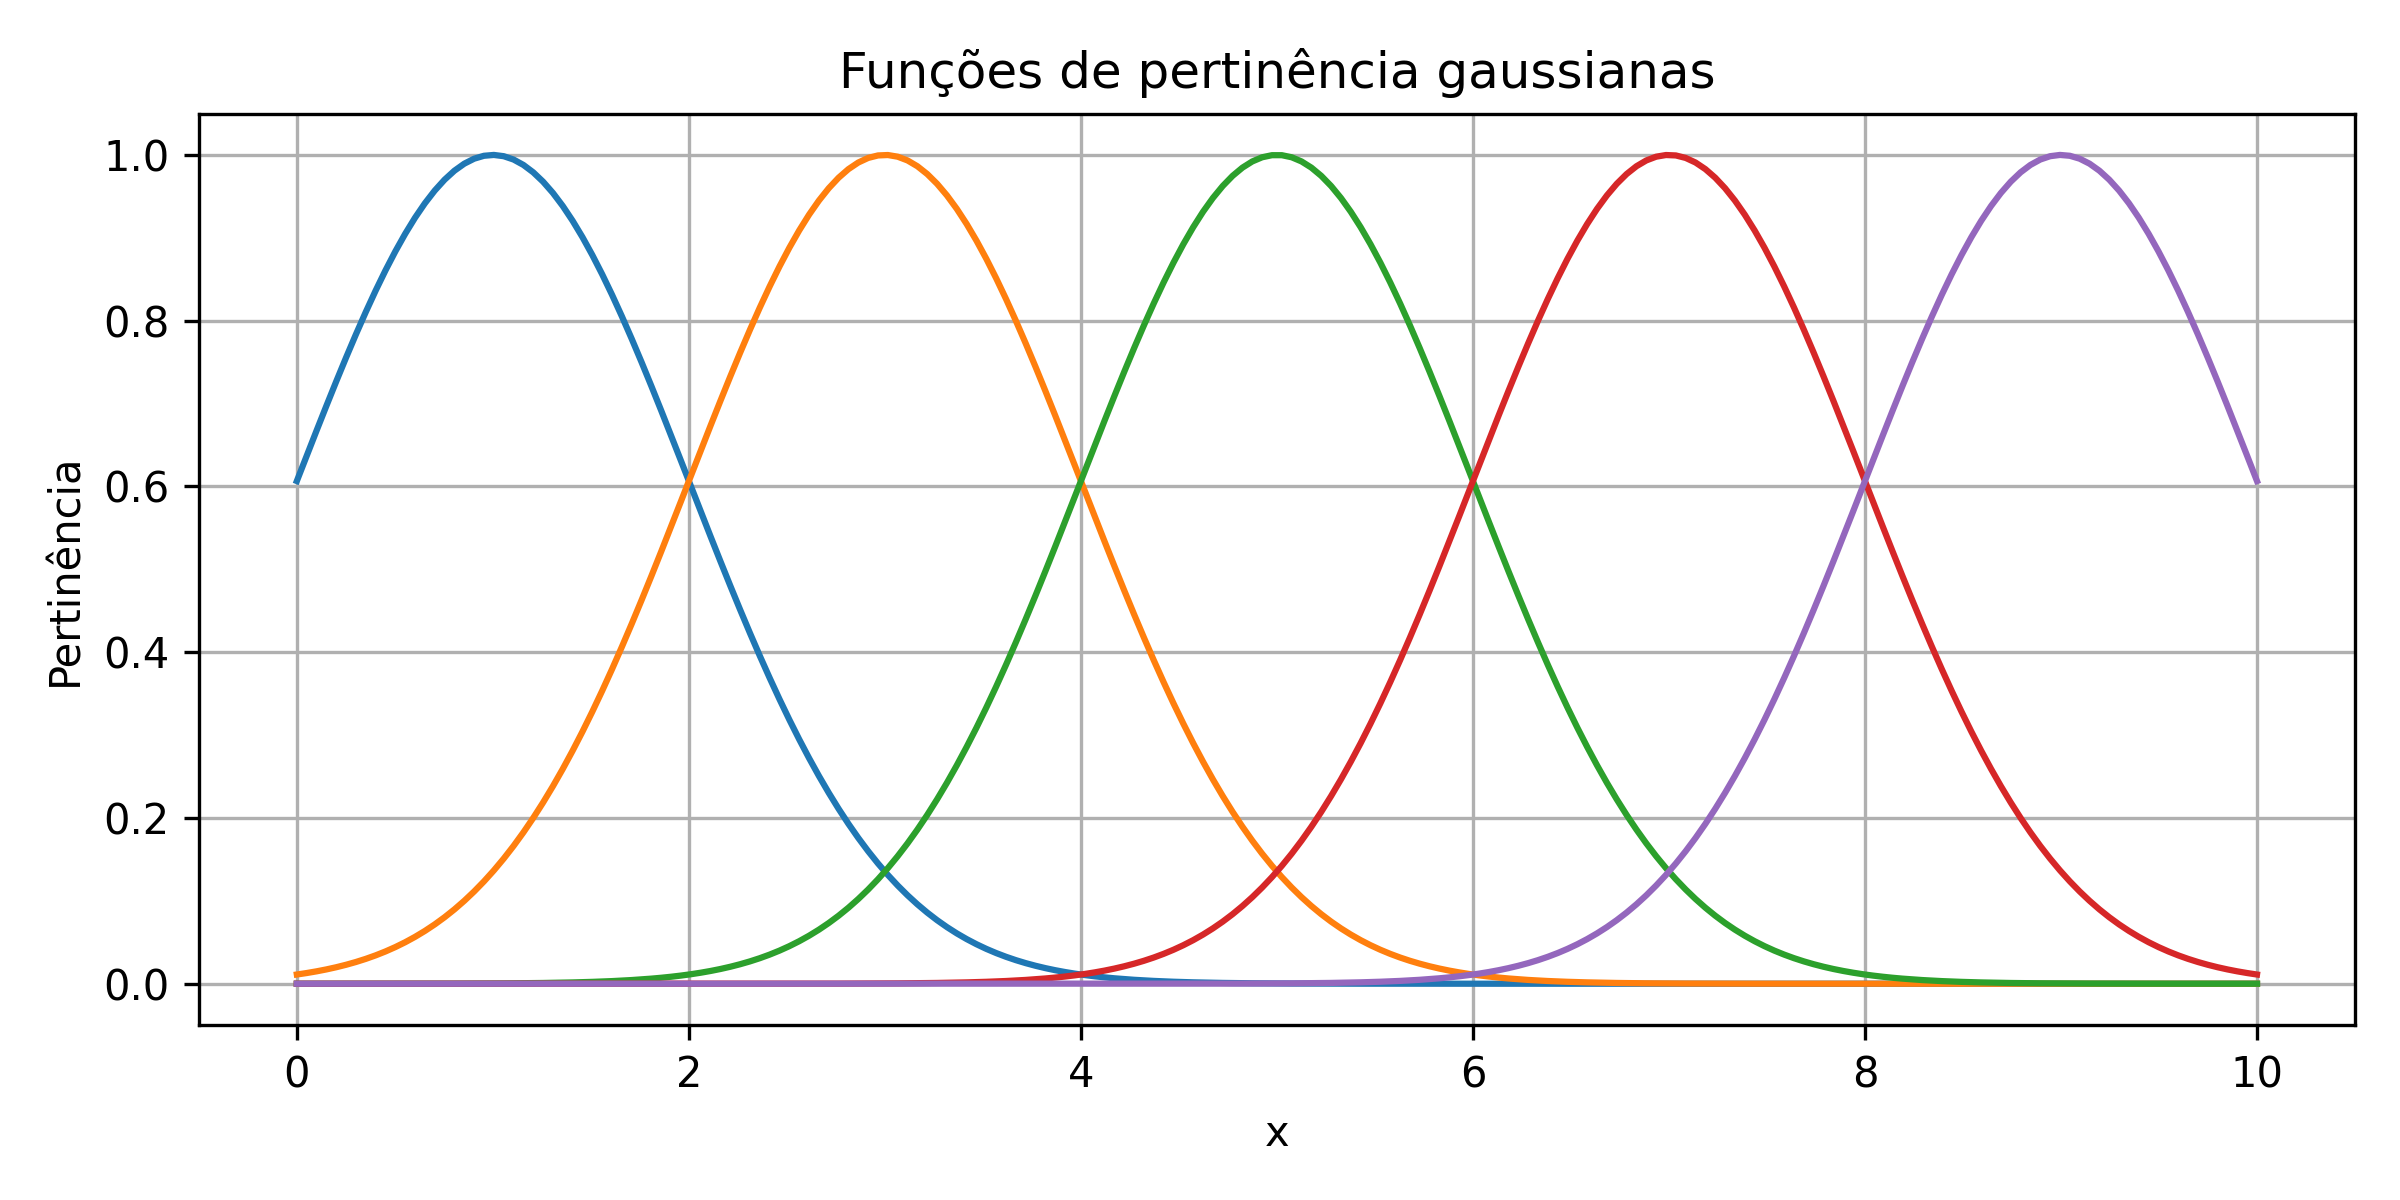
\includegraphics[width=0.45\textwidth]{../img/funcoes_de_pertinencia_gaussianas_5.png}
    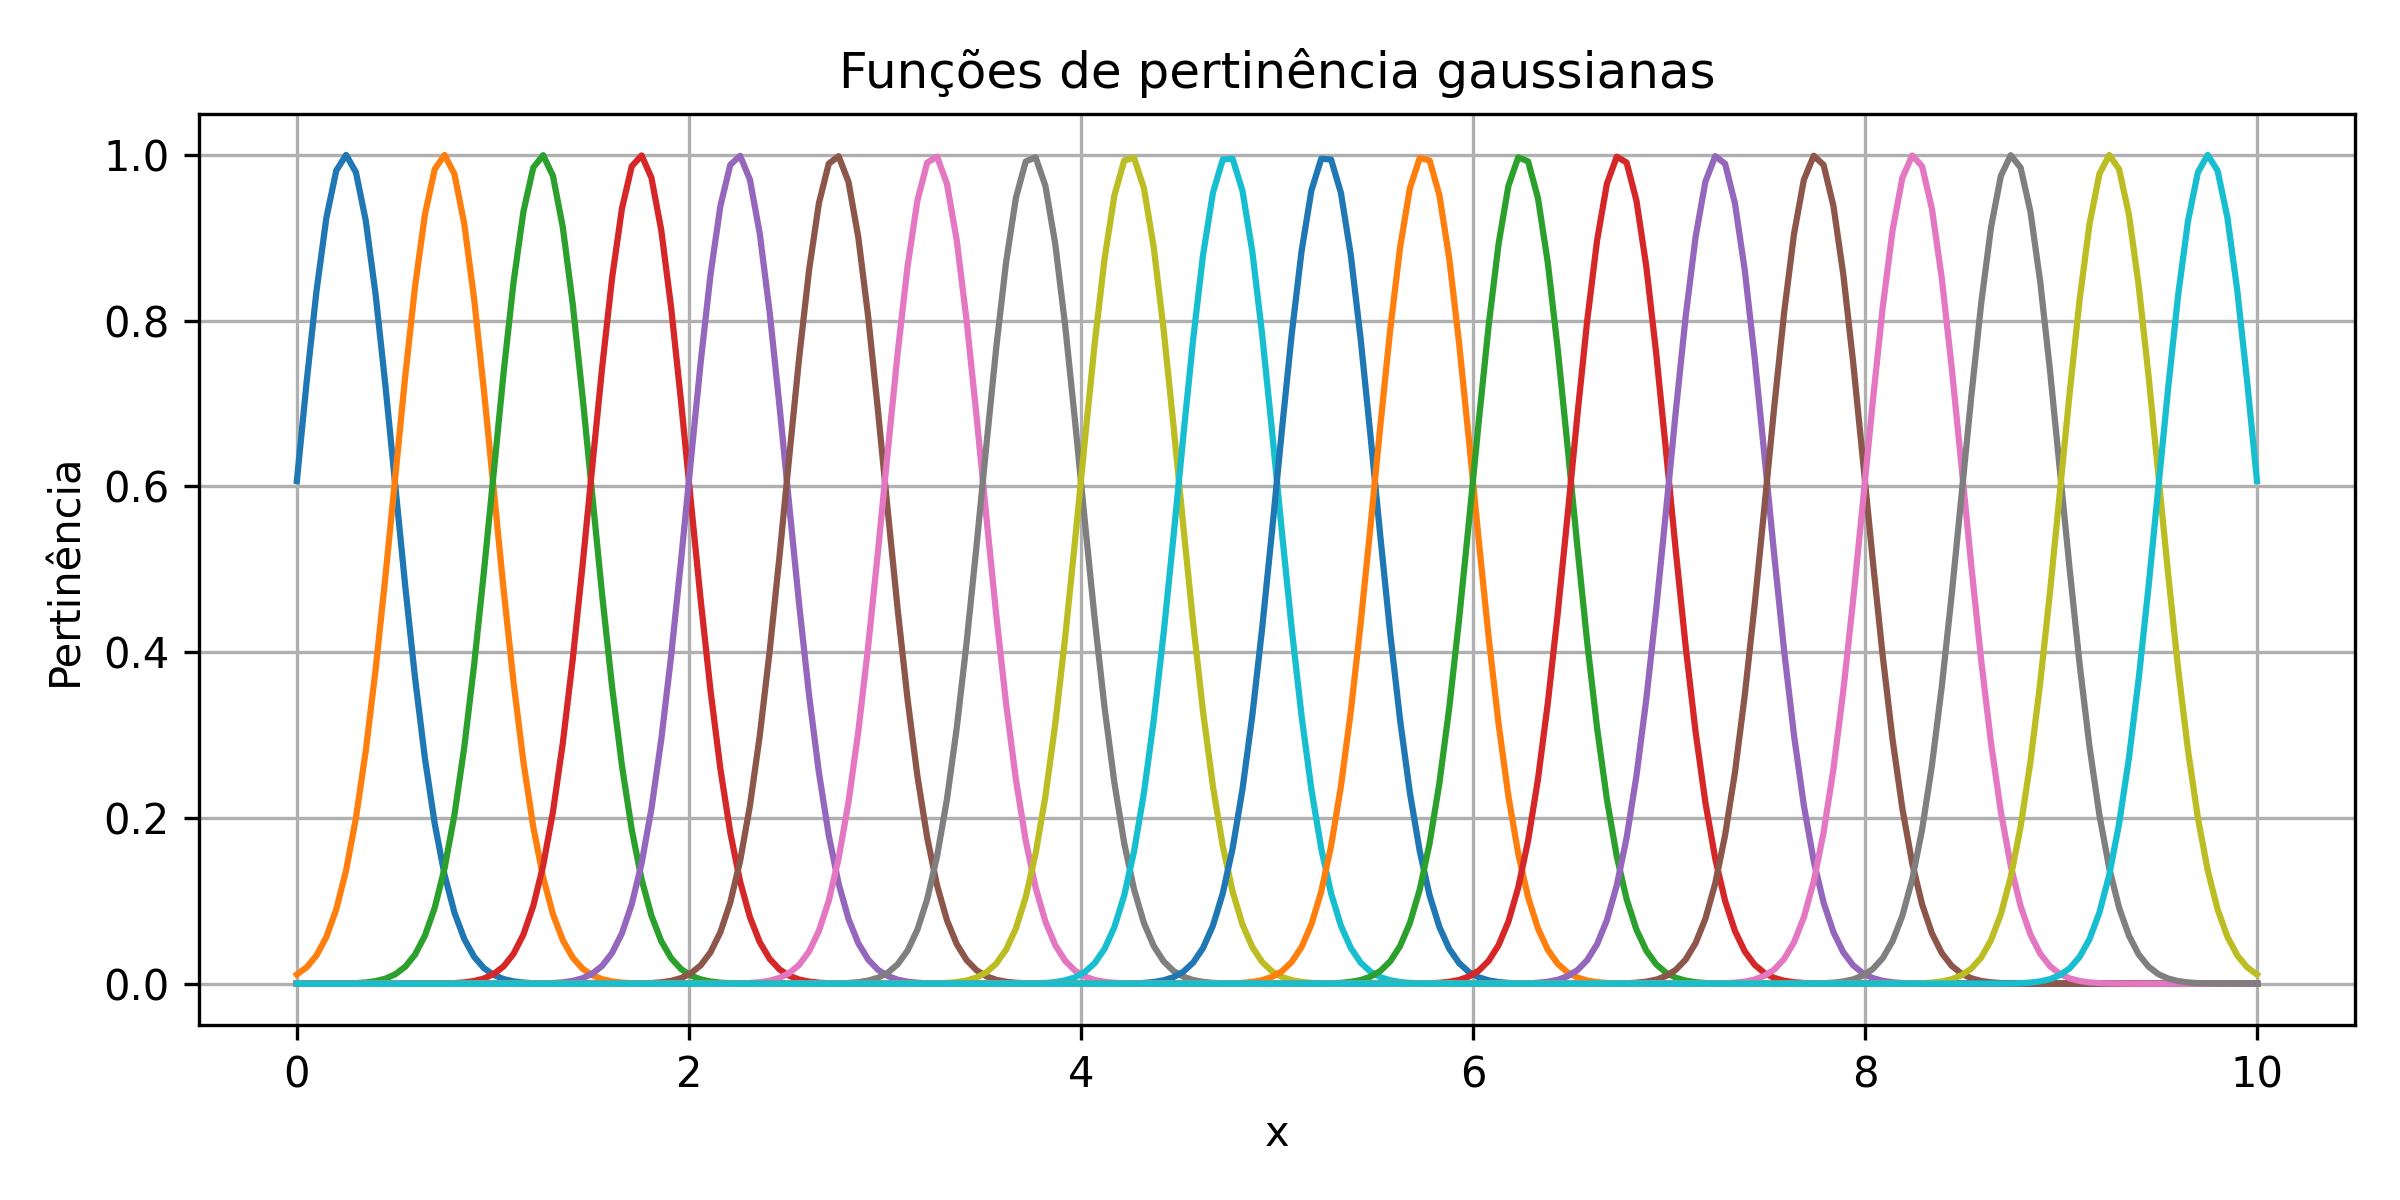
\includegraphics[width=0.45\textwidth]{../img/funcoes_de_pertinencia_gaussianas_20.png}
    \\
    \scriptsize
    \textbf{Esquerda:} Gaussianas ($n_\text{mfs}=5$) \hspace{2em} \textbf{Direita:} Gaussianas ($n_\text{mfs}=20$)
\end{frame}

\begin{frame}{Funções de Pertinência Triangulares e Trapezoidais}
    \centering
    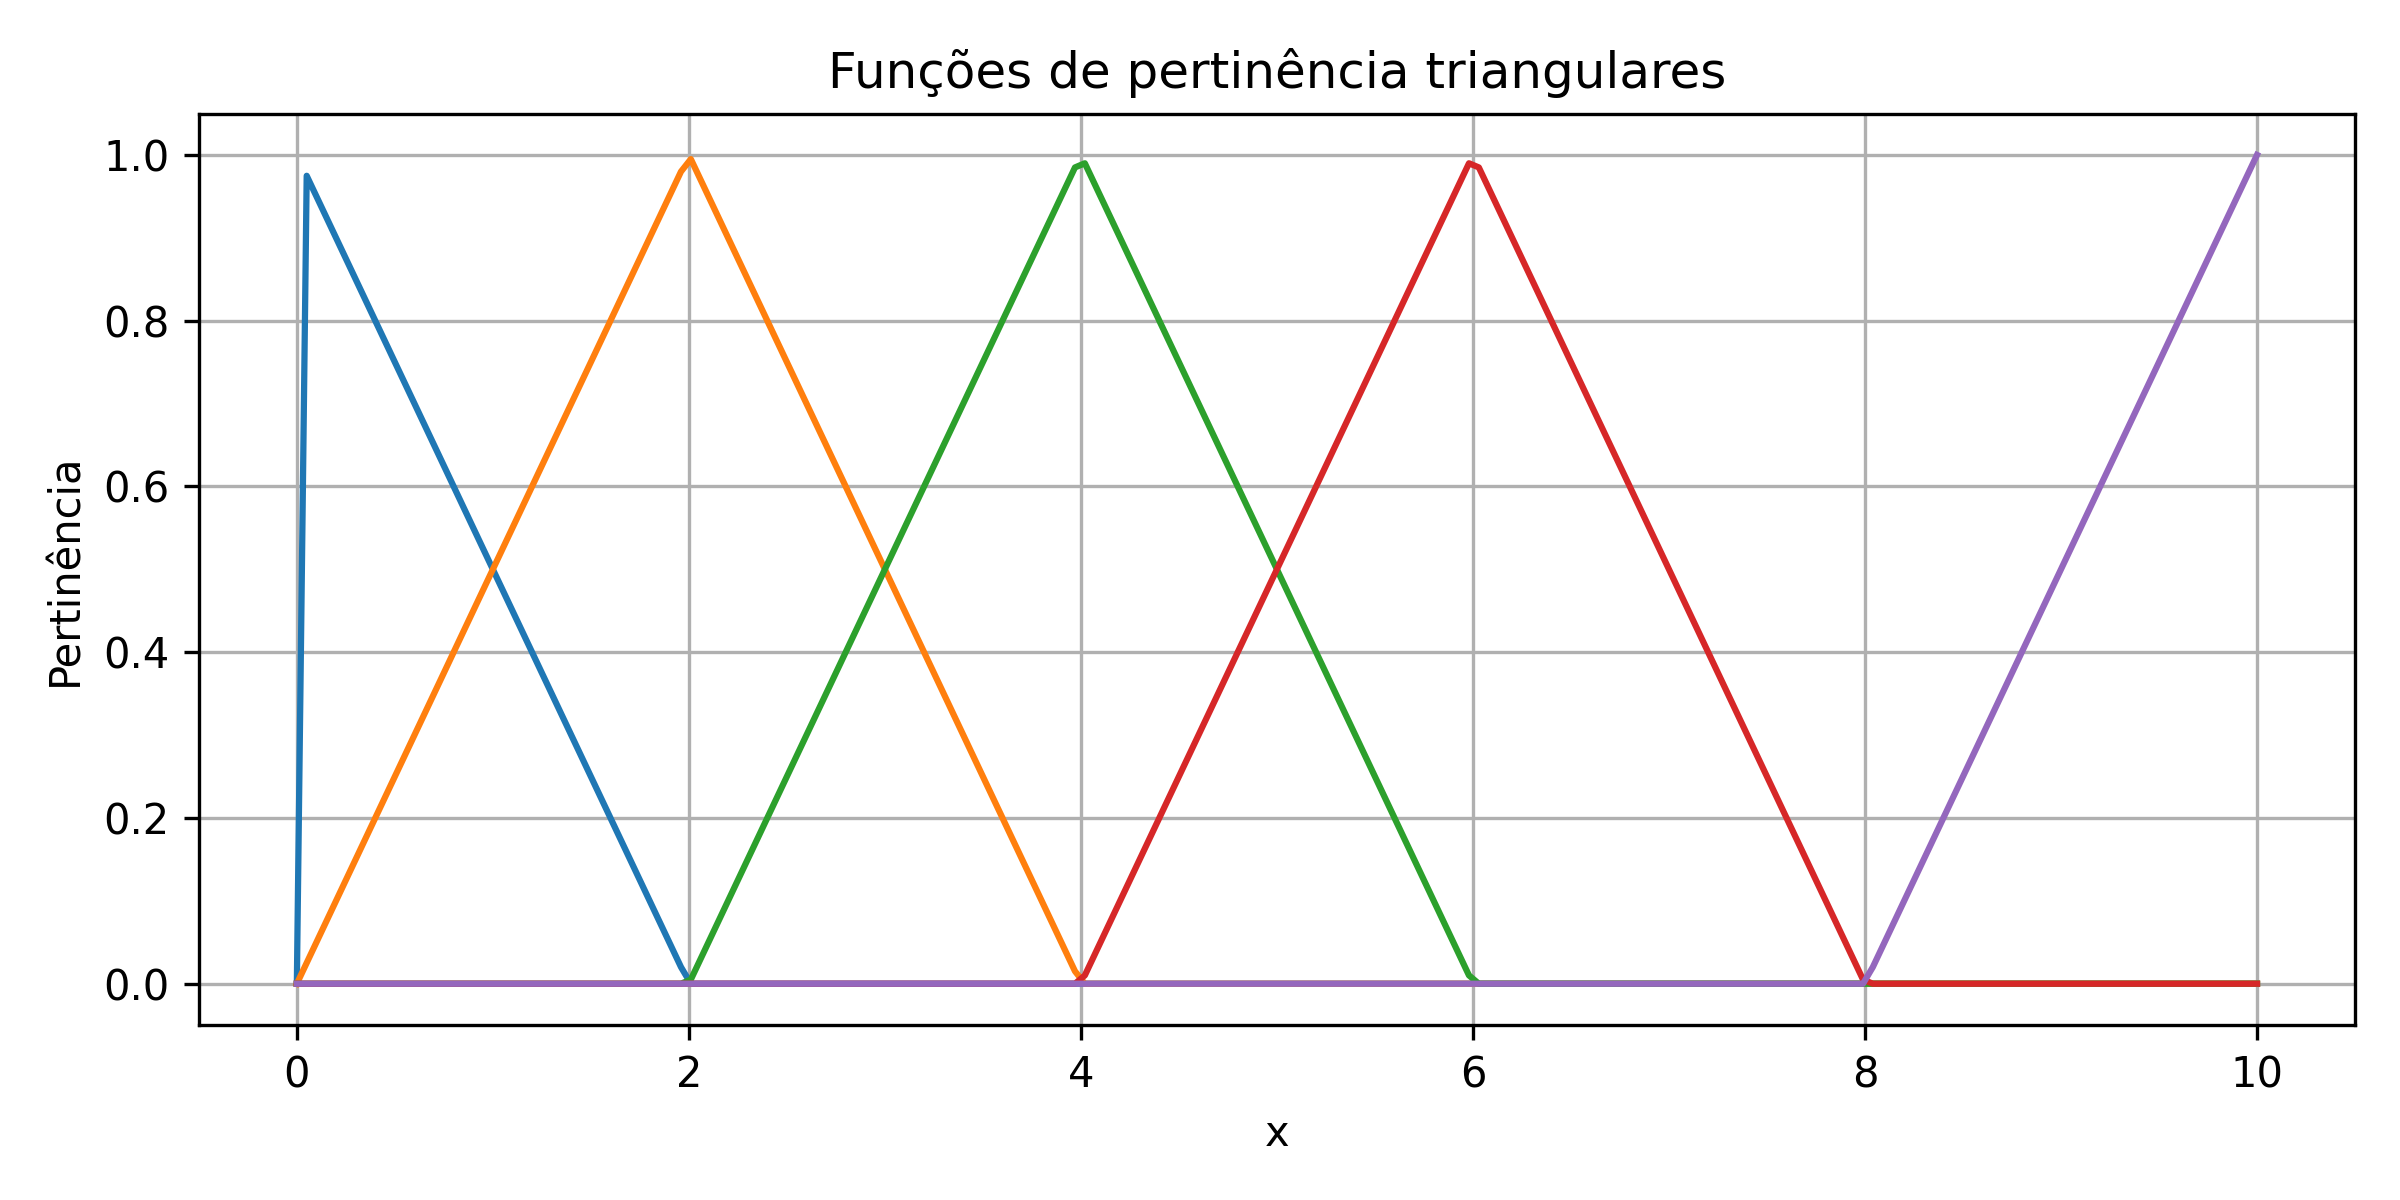
\includegraphics[width=0.45\textwidth]{../img/funcoes_de_pertinencia_triangulares_5.png}
    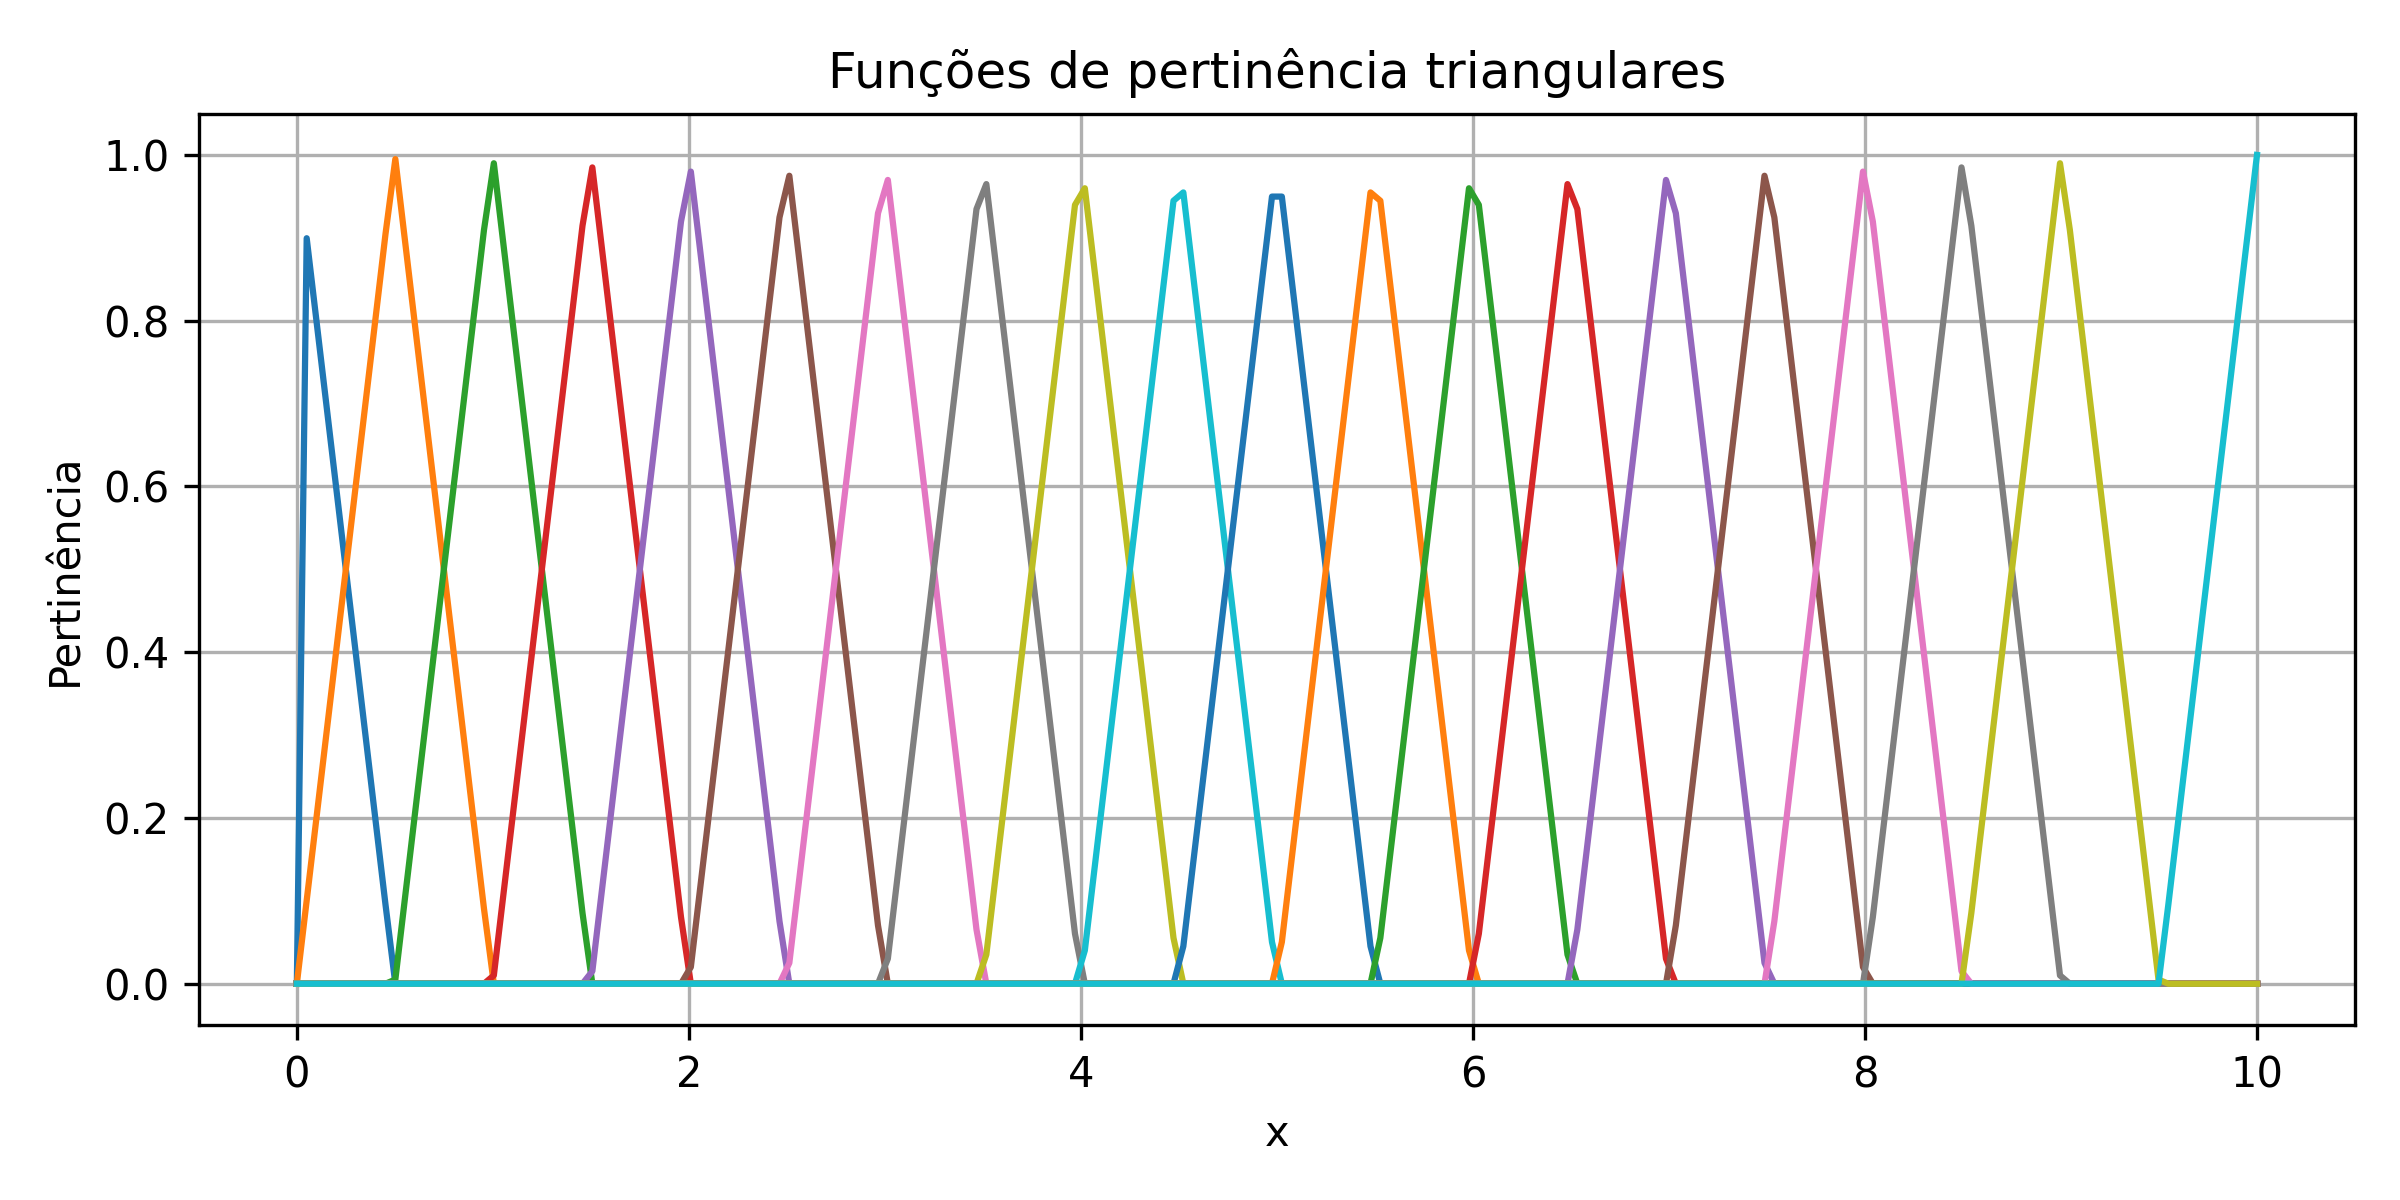
\includegraphics[width=0.45\textwidth]{../img/funcoes_de_pertinencia_triangulares_20.png}
    \\
    \scriptsize
    \textbf{Esquerda:} Triangulares ($n_\text{mfs}=5$) \hspace{2em} \textbf{Direita:} Triangulares ($n_\text{mfs}=20$)
    \vspace{1em}

    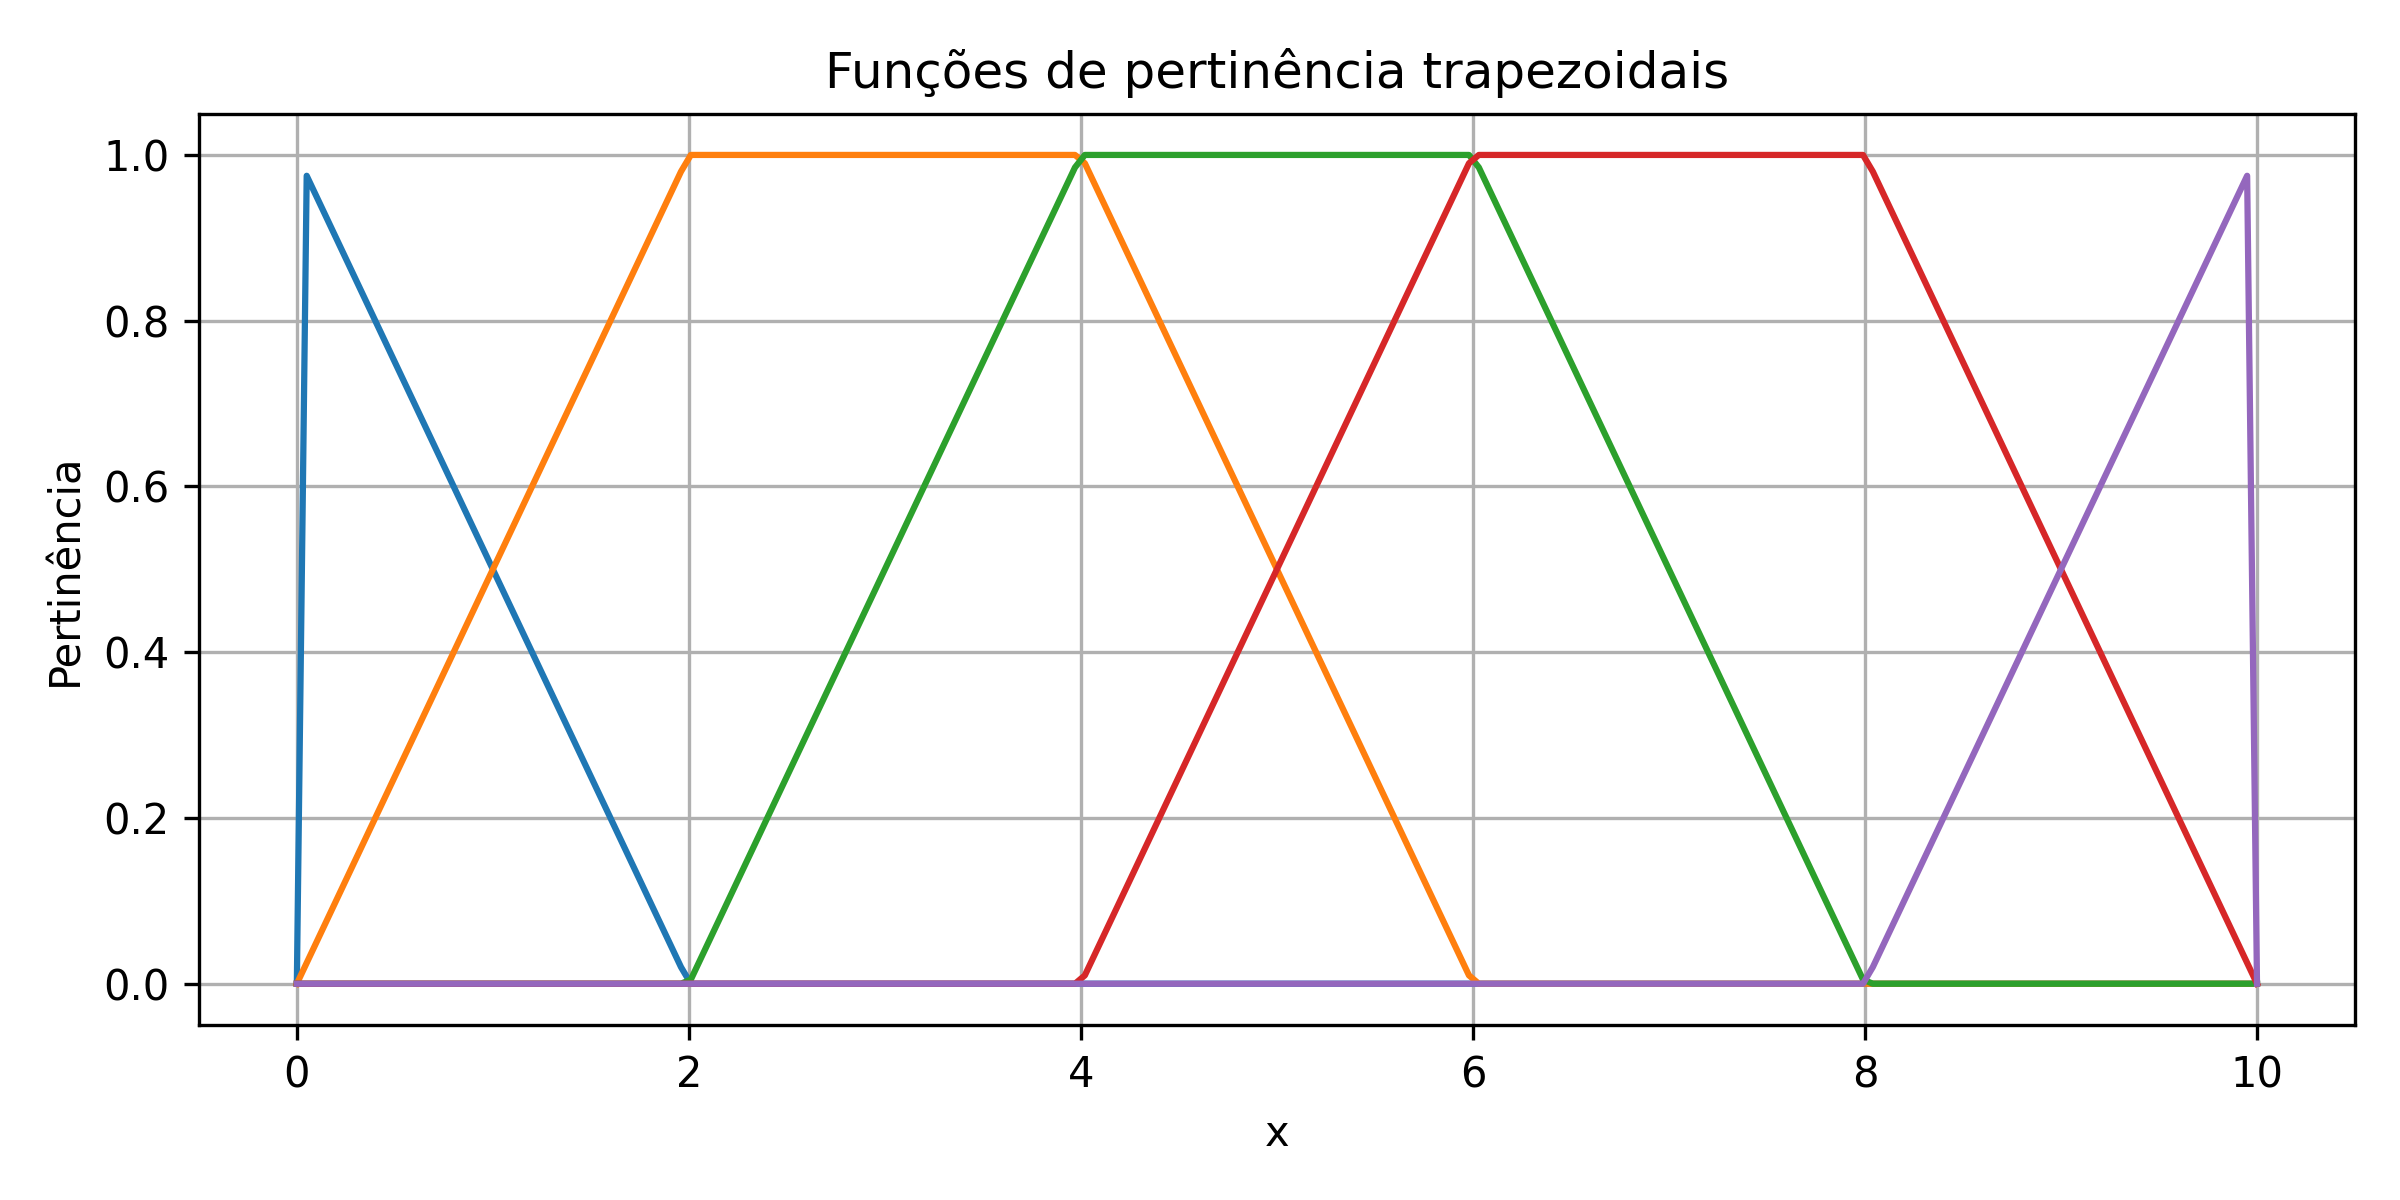
\includegraphics[width=0.45\textwidth]{../img/funcoes_de_pertinencia_trapezoidais_5.png}
    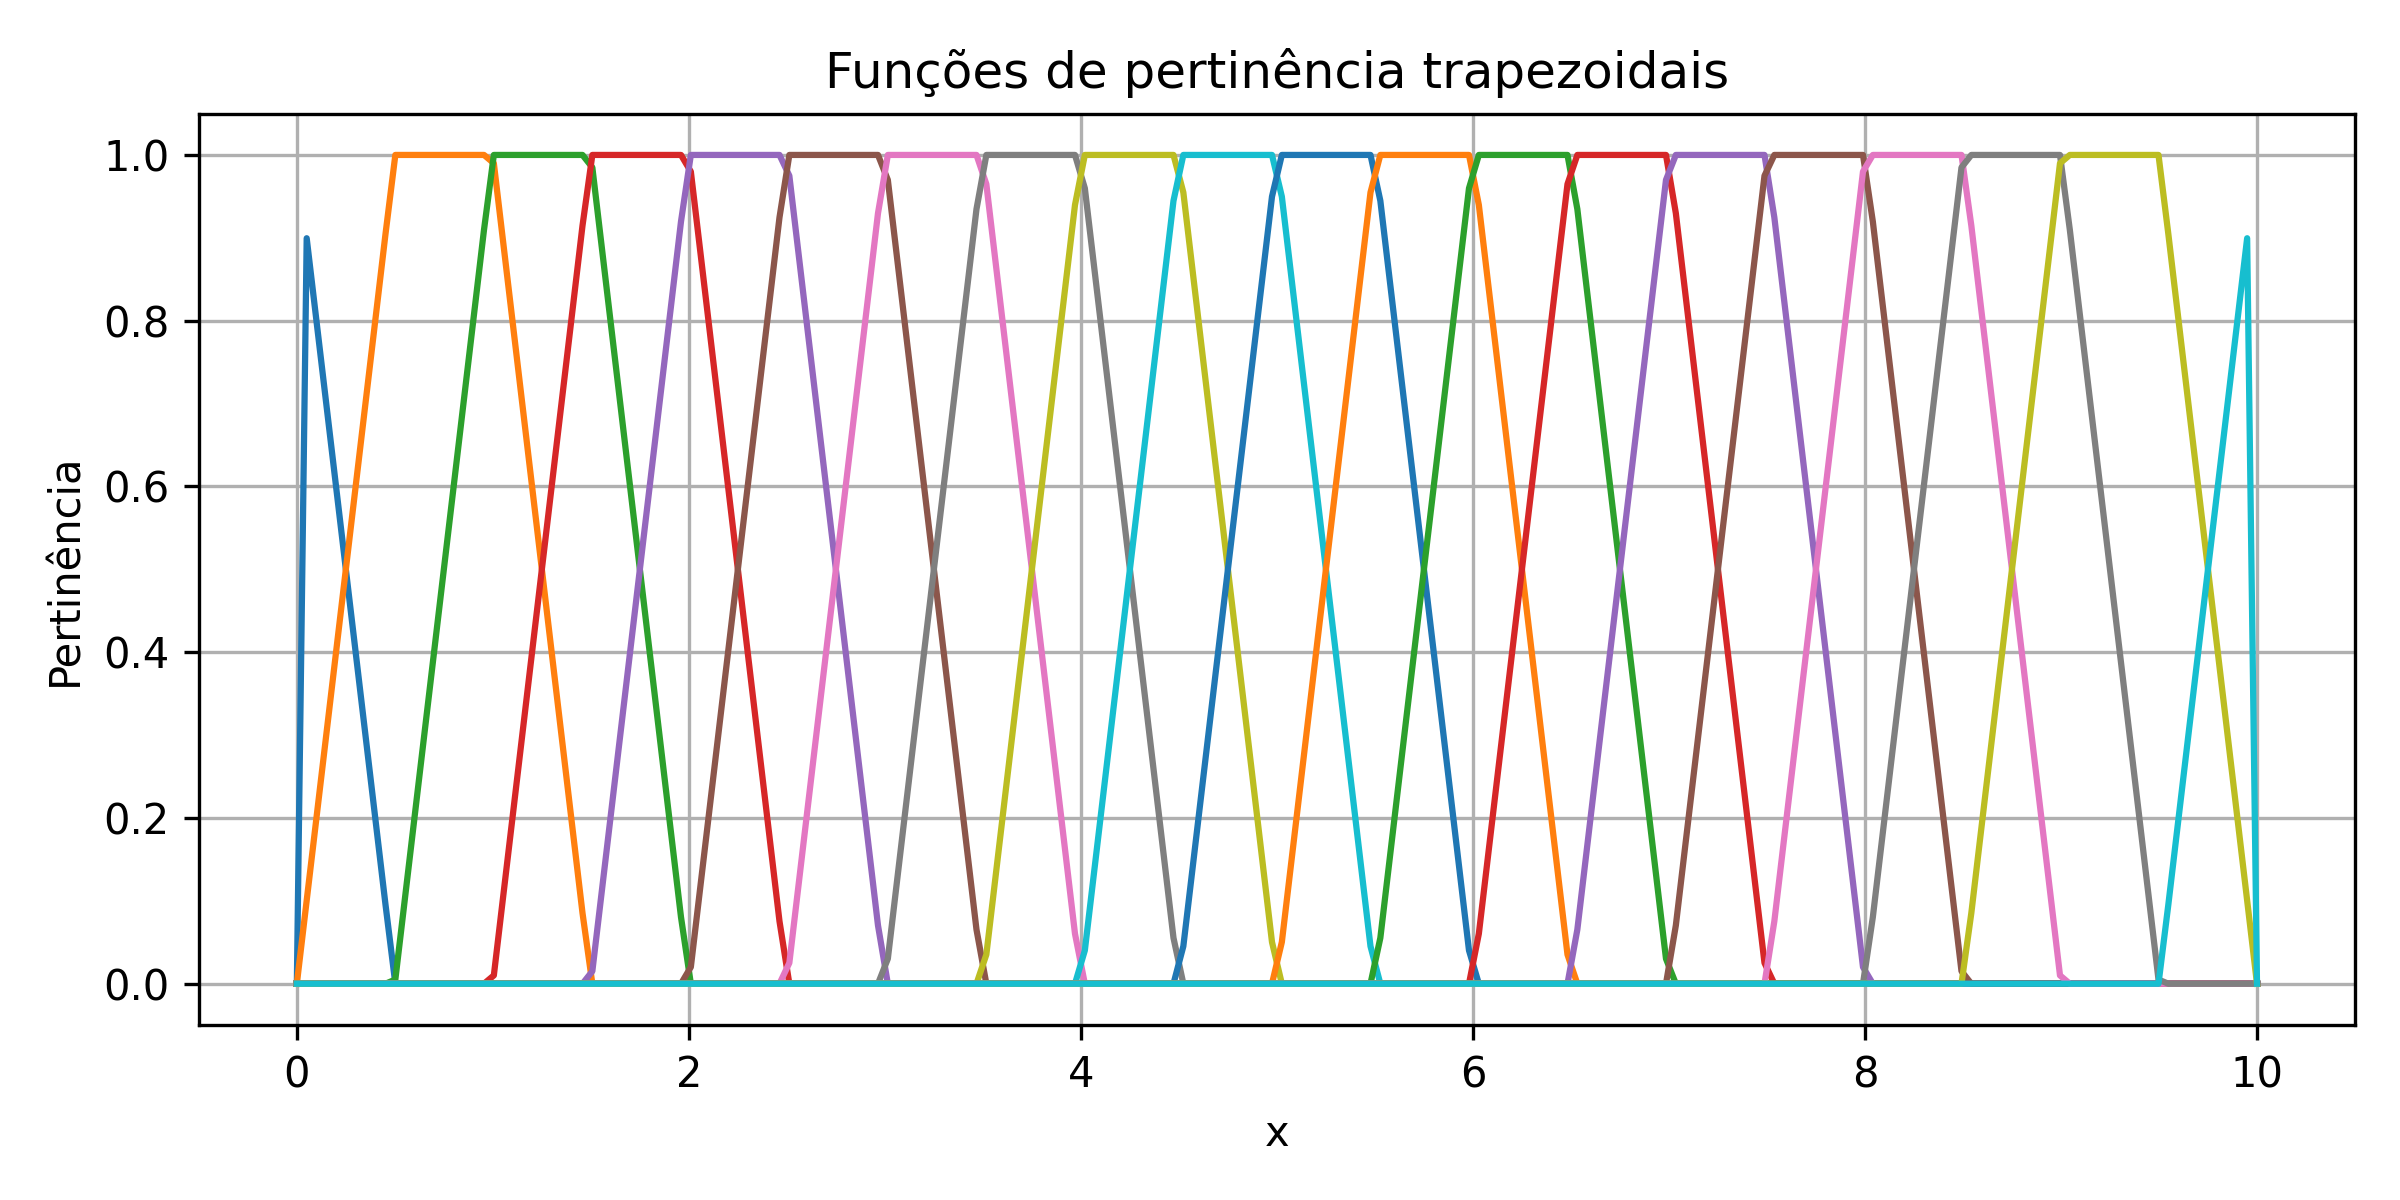
\includegraphics[width=0.45\textwidth]{../img/funcoes_de_pertinencia_trapezoidais_20.png}
    \\
    \scriptsize
    \textbf{Esquerda:} Trapezoidais ($n_\text{mfs}=5$) \hspace{2em} \textbf{Direita:} Trapezoidais ($n_\text{mfs}=20$)
\end{frame}

\section{Resultados e Discussão}

\begin{frame}{Resultados: Antes da Otimização dos Consequentes}
    \begin{itemize}
        \item Antes da otimização, o RMSE já diminui com o aumento de $n_\text{mfs}$ e uso de consequentes lineares.
        \item Para $n_\text{mfs}=5$, RMSE $\approx$ 0.32 (primeira ordem, sem otimização).
        \item Para $n_\text{mfs}=20$, RMSE $\approx$ 0.04 (primeira ordem, sem otimização).
    \end{itemize}
    \vspace{0.5em}
    \begin{columns}
        \column{0.5\textwidth}
        \centering
        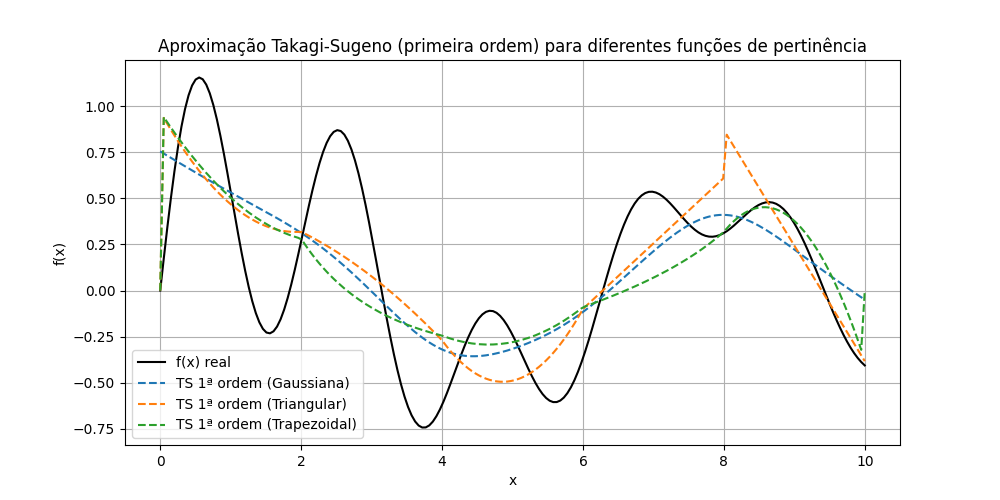
\includegraphics[width=0.95\textwidth]{../img/fx_aprox_1ordem_todas_takagi_sugeno2_5.png}
        \scriptsize
        Aproximação TS 1ª ordem sem otimização ($n_\text{mfs}=5$)
        \column{0.5\textwidth}
        \centering
        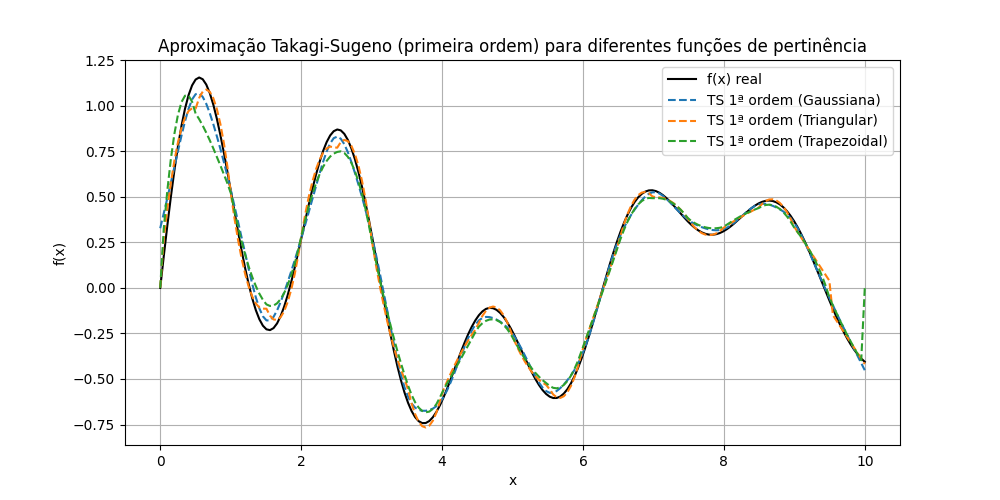
\includegraphics[width=0.95\textwidth]{../img/fx_aprox_1ordem_todas_takagi_sugeno2_20.png}
        \scriptsize
        Aproximação TS 1ª ordem sem otimização ($n_\text{mfs}=20$)
    \end{columns}
\end{frame}

\begin{frame}{Resultados: Após Otimização dos Consequentes}
    \begin{itemize}
        \item A otimização dos consequentes (gradiente descendente) reduz ainda mais o erro.
        \item Para $n_\text{mfs}=5$, RMSE otimizado $\approx$ 0.31 (primeira ordem).
        \item Para $n_\text{mfs}=20$, RMSE otimizado $\approx$ 0.03 (primeira ordem).
    \end{itemize}
    \vspace{0.5em}
    \begin{columns}
        \column{0.5\textwidth}
        \centering
        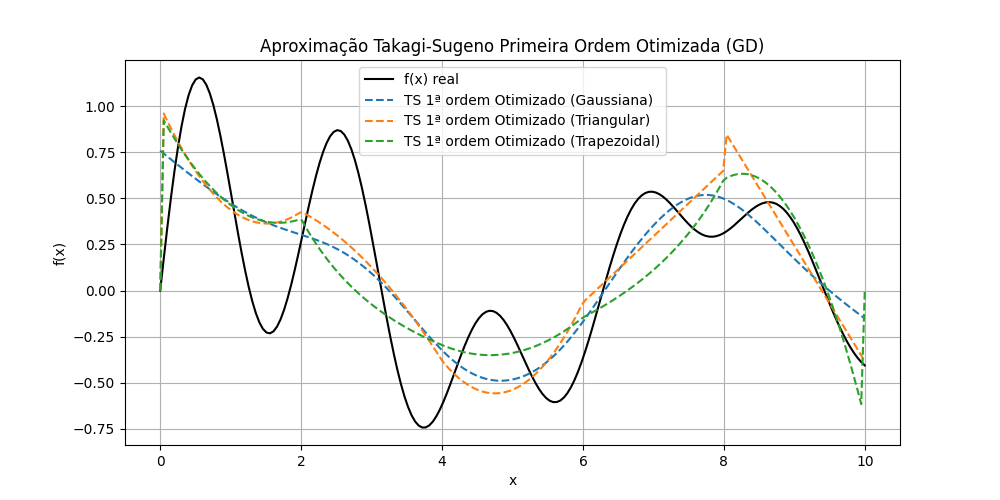
\includegraphics[width=0.95\textwidth]{../img/fx_aprox_1ordem_todas_otimizada_takagi_sugeno2_5.png}
        \scriptsize
        Aproximação TS 1ª ordem otimizado ($n_\text{mfs}=5$)
        \column{0.5\textwidth}
        \centering
        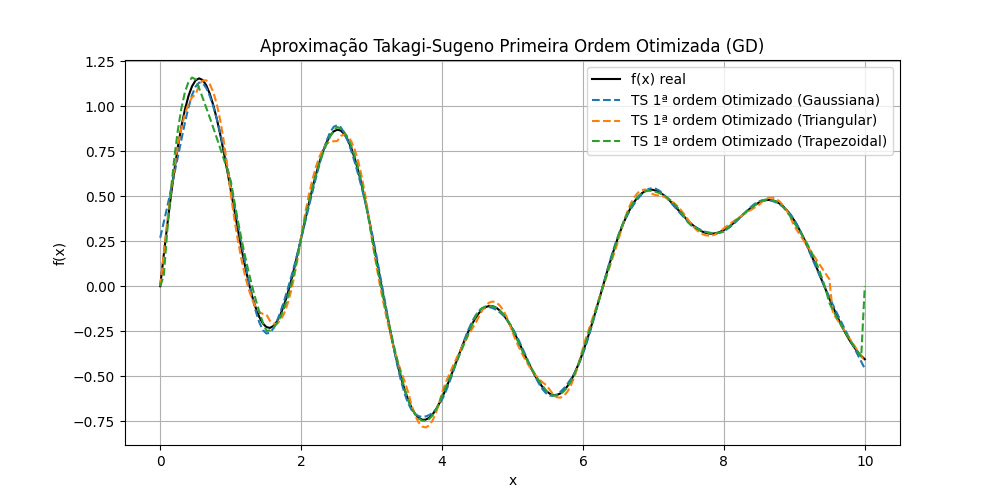
\includegraphics[width=0.95\textwidth]{../img/fx_aprox_1ordem_todas_otimizada_takagi_sugeno2_20.png}
        \scriptsize
        Aproximação TS 1ª ordem otimizado ($n_\text{mfs}=20$)
    \end{columns}
\end{frame}

\begin{frame}{Discussão}
    \begin{itemize}
        \item O aumento do número de funções de pertinência melhora a aproximação, mas aumenta a complexidade.
        \item Consequentes lineares tornam o modelo mais preciso.
        \item Otimização dos consequentes é fundamental para obter baixo erro.
        \item O tipo de função de pertinência influencia o desempenho final.
    \end{itemize}
\end{frame}

\begin{frame}{RMSE dos Modelos Takagi-Sugeno}
    \centering
    \scriptsize
    \textbf{RMSE dos modelos Takagi-Sugeno de ordem zero e primeira ordem, antes e depois da otimização dos consequentes.}
    \vspace{0.5em}
    \begin{tabular}{llcccc}
        \toprule
        $n_\text{mfs}$ & Função & Ordem 0 & Ordem 0 (Opt) & Ordem 1 & Ordem 1 (Opt) \\
        \midrule
        5  & Gaussiana   & 0.38 & 0.34 & 0.33 & 0.31 \\
           & Triangular  & 0.40 & 0.38 & 0.32 & 0.32 \\
           & Trapezoidal & 0.41 & 0.36 & 0.34 & 0.34 \\
        \midrule
        20 & Gaussiana   & 0.16 & 0.08 & 0.05 & 0.03 \\
           & Triangular  & 0.13 & 0.07 & 0.04 & 0.03 \\
           & Trapezoidal & 0.21 & 0.07 & 0.08 & 0.04 \\
        \bottomrule
    \end{tabular}
\end{frame}

\section{Conclusão}

\begin{frame}{Conclusão}
    \begin{itemize}
        \item O sistema Takagi-Sugeno é eficiente para aproximação de funções não lineares.
        \item O desempenho depende do número e tipo de funções de pertinência e do ajuste dos consequentes.
        \item Otimização dos consequentes torna o modelo de ordem zero competitivo com o de primeira ordem.
        \item Para alta precisão, recomenda-se usar mais funções de pertinência e otimização dos parâmetros.
    \end{itemize}
\end{frame}

\begin{frame}{Perguntas?}
    \centering
    \Huge Obrigado!
\end{frame}

\end{document}

